\documentclass{memoriaPFC}

%
% DATOS DEL DOCUMENTO
%

\title{Detector de wifi para Linux}

%\autores{Nombre1 Apellidos1}{Nombre2 Apellidos2}
\autores{Jos� Chorva Aguilella}{}

\director{Juan Echag�e Guardiola}
%\directora{Ursula K. Le Guin}

% iaei ii ioi itel
\titulacion{itis}

% mayo || septiembre (en min�sculas!!)
\date{junio de 2011}

\resumen{%
Hoy en d�a, el est�ndar IEEE 802.11, m�s conocido por Wifi se ha popularizado en las redes dom�sticas. La comodidad que supone no tener cables en los ordenadores, principalmente port�tiles, permite un mejor traslado de los equipos inform�ticos, ya que es com�n disponer de tomas de corriente el�ctrica en pr�cticamente todas las paredes de una casa u oficina, pero no suelen encontrarse equipadas de tomas ethernet.\\

La creaci�n de Interfaces gr�ficas tiene una gran relevancia a la hora de interactuar con un programa, permitiendo incluso, un mayor entendimiento de los datos a analizar. En el desarrollo de interfaces es importante tener en cuenta la funcionalidad del programa frente a querer mostrar todos los datos sin aparente criterio o de tener que recurrir a comandos de consola para seleccionar los datos que nos interesen en un momento determinado.\\

Este proyecto ofrece una interfaz gr�fica intuitiva para analizar las principales caracter�sicas de una red inal�mbrica, como son la potencia de la se�al y el canal por el que transmiten. As� pues, la usabilidad de �ste proyecto es un factor clave para un correcto an�lisis de las redes Wifi presentes en el entorno. \\


}
\descriptores{wifi, redes, monitorizaci�n}


%\newcommand{\wifi}{WifiScan }
%\newcommand{\Wifi}{Wi-Fi }
%\newcommand{\gui}{interaz gr�fica }
%\newcommand{\guis}{interfaces gr�ficas }


%
% COMIENZO DEL DOCUMENTO
%
\begin{document}

% Portada, resumen, indices
\frontmatter
\hacerportada
\hacerresumen
\tableofcontents
\listoffigures % Opcional
\listoftables % Opcional
%\listoflistings % Opcional

% Contenidos
\mainmatter


\chapter{Introducci�n}
\section{Motivaci�n}

Durante la instalaci�n de redes inal�mbricas, es importante verificar que la se�al llega correctamente hasta el lugar que nos interese, y que las interferencias causadas por las redes colindantes sean las m�nimas posibles, para que la transmisi�n sea lo m�s eficiente posible.\\

Un esc�ner de redes inal�mbricas permite solucionar de problemas de una red existente o analizar cual o cuales llegan con m�s potencia a nuestro receptor. Permite tambi�n realizar una auditor�a preliminar de la seguridad de la red seleccionada, averiguando si tiene alg�n mecanismo de protecci�n (contrase�a o encriptacion).\\

Tambi�n permite saber cu�ntas redes hay en el entorno y la potencia de sus se�ales, para verificar la cobertura wifi de un determinado espacio, evaluar la posibilidad de roaming, la presencia de interferencias de radiofrecuencia o `puntos muertos'', y la ubicaci�n �ptima de los puntos de acceso y las antenas.\\


Una herramienta de diagn�stico corresponder�a a la categor�a de esc�neres WiFi. El m�s conocido de esta categor�a es NetStumbler. Una herramienta de informes de cada red inal�mbrica que detecta, junto con el canal utilizado por el punto de acceso (AP), la potencia de la se�al recibida\ldots \\

Aproximadamente cada 100 ms un punto de acceso env�a una se�al y la tarjetas receptoras inal�mbrica 802.11, tambi�n conocidas como tarjetas wifi o ``wifis'' las detectan, y a�aden el SSID a su lista de redes inal�mbricas conocidas. Adem�s, es posible obtener los informes para cada AP individualmente, es decir, los que recibe en su ubicaci�n actual. Esto permite la combinaci�n con un receptor de GPS para realizar mapas de redes inal�mbricas. Esto es �til para grandes superficies donde es necesaria la cobertura Wifi en todo el recinto o recorrido.\\



\section{IEEE 802.11}


Hoy en d�a, el est�ndar IEEE 802.11, m�s conocido por Wifi se ha popularizado en las redes dom�sticas. La comodidad que supone no tener cables en los ordenadores, principalmente port�tiles, permite un mejor traslado de los equipos inform�ticos, ya que es com�n disponer de tomas de corriente el�ctrica en pr�cticamente todas las paredes de una casa u oficina, pero no suelen encontrarse equipadas de tomas ethernet.\\

Tambi�n es m�s sencilla la conexi�n de varios ordenadores, ya que no se est� tan limitado de recursos (por ejemplo, disponer de un router de 4 puertos ethernet y tener 5 ordenadores). Con Wifi es posible conectar hasta 254 equipos a la misma red sin necesidad de hacer un gasto extra en infraestructuras.\\

%%LOGO WIFI
\figura{0.4}{imgs/capturas/wifilogo.png}{Logotipo de wifi}{}{h}


El est�ndar Wifi dispone de varias especificaciones (a, b, g \ldots), siendo el est�ndar IEEE802.11n ratificado por IEEE en 2009 como el m�s actual de esta tecnolog�a. Este est�ndar tiene una velocidad de 600 Mbps en la capa f�sica, tiene compatibilidad con todos los est�ndares anteriores y puede trabajar en dos bandas de frecuencias, 2,4 GHz o 5 GHz. Y gracias a la tecnolog�a MIMO (Multiple Input	-- Multiple Output), puede operar en varios canales a la vez para una mejor transmisi�n de datos mediante la incorporaci�n de varias antenas.\\

Un punto de acceso inal�mbrico (WAP) se conecta a un grupo de dispositivos inal�mbricos a un lado por cable LAN . Un punto de acceso se asemeja a un hub, la transmisi�n de datos entre los dispositivos inal�mbricos conectados, adem�s de un solo dispositivo conectado por cable, m�s a menudo un hub o switch Ethernet, permitiendo que los dispositivos inal�mbricos para comunicarse con otros dispositivos con cable.\\

%%RED WIFI
\figuraSinMarco{0.4}{imgs/capturas/WLAN.png}{ejemplo de red inal�mbrica}{}{h}


Los adaptadores inal�mbricos permiten que los dispositivos para conectarse a una red inal�mbrica. Estos adaptadores se conectan a los dispositivos con varias interconexiones internas o externas, tales como PCI , miniPCI , USB , ExpressCard , y Cardbus PC Card . A partir de 2010 , la mayor�a de los nuevos ordenadores port�tiles vienen equipados con adaptadores internos. \\

Los routers inal�mbricos integran un punto de acceso inal�mbrico, Ethernet switch, y la aplicaci�n interna del firmware del router que proporciona IP routing , NAT y DNS de reenv�o a trav�s de un sistema integrado de interfaz WAN. Un router inal�mbrico permite red cableada e inal�mbrica con dispositivos Ethernet LAN para conectarse a un (por lo general) solo dispositivo WAN, tal como un m�dem de cable o m�dem DSL . Un router inal�mbrico permite a los tres dispositivos, principalmente el punto de acceso y el router, que se configura a trav�s de una central de servicios p�blicos. Esta utilidad es por lo general un sistema integrado de servidor web que sea accesible para los clientes inal�mbricos y con cable LAN y, opcionalmente, a menudo a los clientes WAN. \\
	
%%ROUTER WIRELESS
\figura{0.5}{imgs/capturas/router.png}{Router wifi}{}{h}
	
	
Los bridges wireless pueden conectar una red cableada a una red inal�mbrica. Un bridge es distinto de un punto de acceso: un punto de acceso conecta dispositivos inal�mbricos a una red cableada en la capa de enlace de datos . Dos bridges inal�mbricos pueden ser utilizados para conectar dos redes de cable sobre un enlace inal�mbrico, �til en situaciones donde una conexi�n por cable puede no estar disponible, por ejemplo, entre dos casas separadas.\\

%%BRIDGE
\figuraSinMarco{0.6}{imgs/capturas/bridge.png}{Bridge wireless}{}{h}


Los extensores o repetidores inal�mbricos pueden ampliar el alcance de una red inal�mbrica existente. Estrat�gicamente colocados pueden alargar un �rea de se�al o permitir ampliar el �rea de la se�al para superar obst�culos tales como los relacionados a corredores o edificios en forma de L. Los dispositivos inal�mbricos conectados a trav�s de repetidores sufren un periodo de latencia para cada dispositivo. Adem�s, un dispositivo m�vil conectado a cualquiera de los repetidores de la cadena tendr� una producci�n limitada por el "eslab�n m�s d�bil" entre los dos nodos en la cadena de la cual se origina la conexi�n a donde finaliza la conexi�n.\\

%%REPETIDOR WIFI
\figuraSinMarco{0.6}{imgs/capturas/repetidor.jpg}{Esquema de uso de un repetidor}{}{h}


\section{Objetivos y herramientas}

La herramienta de desarrollo (en adelante, Wifi) desarrollada en este proyecto est� basada en el programa para Microsoft Windows NetSurveyor\footnote{http://www.performancewifi.net/performance-wifi/products/netsurveyor-network-discovery.htm}. Este proporciona informaci�n gr�fica de las distintas redes detectadas y permite una interpretaci�n casi intuitiva de sus datos. \\

El objetivo principal de �ste proyecto es ofrecer una interfaz gr�fica para combinar herramientas de an�lisis de redes inal�mbricas con otras de muestreo estad�stico, utilizando una plataforma de desarrollo multiplataforma para tener la opci�n de hacer versiones para otros sistemas operativos.\\

La creaci�n de Interfaces gr�ficas tiene una gran relevancia a la hora de interactuar con un programa, permitiendo incluso, un mayor entendimiento de los datos a analizar. En el desarrollo de interfaces es importante tener en cuenta la funcionalidad del programa frente a querer mostrar todos los datos sin aparente criterio o de tener que recurrir a comandos de consola para seleccionar los datos que nos interesen en un momento determinado.\\

La usabilidad de �ste proyecto es un factor clave para un correcto an�lisis de las redes Wifi presentes en el entorno. Es importante que los elementos clave (los datos de las redes) est�n en todo momento a la vista del usuario de la aplicaci�n, esto permitir� una visualizaci�n m�s intuitiva de ellas.\\

Otro factor a tener en cuenta es la plataforma en que se va a utilizar la aplicaci�n. Debido a la multitud de dispositivos con receptores Wifi integrados (PDAs, m�viles, netbooks\ldots), es conveniente una herramienta que sea f�cil de usar y que tenga opci�n de ser utilizada en otras plataformas.\\

Las herramientas utilizadas en �ste proyecto han sido;
\begin{itemize}
\item Wireless Tools, concretamente iwlist
\item GnuPlot
\item Qt
\item \LaTeX
\end{itemize}

Las principales ventajas de utilizar herramientas libres externas al programa son la facilidad de mantener el c�digo actualizado ante posibles errores ``bugs'' de �stas, ya que al ser herramientas muy extendidas, tienen una comunidad de desarrollo y soporte muy amplio y permiten mantener actualizado el software.\\




\chapter{Herramientas utilizadas}
\section{Wireless Tools}
Wireless Tools es un paquete de herramientas de verificaci�n y configuraci�n de redes Wifi, sus principales aplicaciones son \texttt{iwconfig, iwlist, iwspy, iwpriv, iwgetid, ifrename e iwevent}. La herramienta utilizada en el desarrollo del proyecto ha sido iwlist.\\
 Iwlist se utiliza para mostrar informaci�n adicional de las interfaces de redes inal�mbricas detectadas. El principal argumento se utiliza para seleccionar una categor�a de informaci�n, iwlist muestra en forma detallada toda la informaci�n relacionada con esta categor�a.\\

\textbf{Par�metro scan}
Devuelve la lista de puntos de acceso y celdas Ad-Hoc dentro de rango y, opcionalmente, informaci�n sobre ellos (ESSID, calidad, frecuencia, modo \ldots). El tipo de informaci�n devuelta depende de lo que admite la tarjeta, generalmente muestra la direcci�n MAC del punto de acceso, su nombre de red o ESSID, canal en que realiza la transmisi�n, ratio de transferencia y la encriptaci�n de la red.

\subsection{Ejemplo}
Por medio de la captura de datos de una red, se explicar� el significado de cada campo obtenido:

\begin{itemize}
\item wlan0     Scan completed :
Esto significa que ha realizado el escaneo de datos y ha encontrado al menos una red, en caso contrario, mostrar�a:
\item wlan0     No scan results
\end{itemize}
Una vez clasificadas las redes encontradas, las separa en celdas (Cells), aqu� podemos ver un ejemplo de una red:\\

\lstinputlisting[language=bash,caption={Ejemplo de iwlist scan}]{src/iwlistscan.sh}



\section{GnuPlot}
\subsection{Generaci�n de gr�ficos}
%%%%%%%%%%%%%%%%%%%%%%%%%
Gnuplot es un programa de l�nea de comandos que puede generar gr�ficos de funciones en dos y tres dimensiones. Se utiliza con frecuencia para los gr�ficos con calidad de publicaci�n, as� como los prop�sitos educativos. Gnuplot puede producir una salida directamente en la pantalla, o en muchos formatos de archivos gr�ficos, incluyendo Portable Network Graphics (PNG), PostScript encapsulado (EPS), Scalable Vector Graphics (SVG), JPEG y muchos otros. El programa puede ser utilizado tanto de forma interactiva y en modo batch utilizando scripts.\\
%%%%%%%%%%%%%%%%%%%%%%%%%
Fue creado originalmente para permitir a los cient�ficos y los estudiantes a visualizar funciones matem�ticas y datos de manera interactiva, pero ha crecido para apoyar muchas aplicaciones no interactivas, tales como secuencias de comandos web. Tambi�n se utiliza como un motor de trazado por las aplicaciones de terceros como octava. Gnuplot ha contado con el apoyo y bajo desarrollo activo desde 1986.\\

Gnuplot es compatible con muchos tipos diferentes de salida: pantalla de los terminales interactivos (con tecla de acceso directo y la entrada del mouse), salida directa a plotters o impresoras modernas, y la salida a muchos formatos de archivo (eps, fig, jpeg, LaTeX, metafont, PBM, pdf, png , PostScript, SVG, \ldots). \\

\section{Qt}
\subsection{Descripci�n de Qt}
Las librerias gr�ficas de Qt fueron desarrolladas para disponer de un GUI para C++ multiplataforma por la compa�ia Trolltech. Qt cambi� a licencia GPL en el a�o 2000, siendo gratuita para el software libre y de pago para el privativo, a 
partir de la compra de Trolltech por parte de Nokia en 2008.\\

%\figura{0.4}{imgs/capturas/qt-logo.jpg}{Logotipo de Qt}{}{}

\figuraSinMarco{0.4}{imgs/capturas/qt-logo.jpg}{Logotipo de Qt}{Logoqt}{h}

Qt fue utilizada para el desarrollo de KDE entre 1996 y 1998, y �ste se convirti� en un escritorio muy popular entre la comunidad GNU/Linux. Esto provoc� la aparici�n del escritorio GNOME con GTK+ debido a que la licencia de Qt se basaba en software propietario. En 1998 los desarrolladores de KDE y Trolltech establecieron la KDE Free Qt Foundation, la cual permit�a liberar la biblioteca Qt bajo una licencia tipo BSD10.En el a�o 2000, Trolltech pas� a ofrecer la biblioteca Qt bajo GPL para la versi�n Linux, en Mac OS X se publico en 2003 y en MS Windows en 2005. \\

Actualmente, Qt cuenta con tres tipos de licencia; 
\begin{itemize}
\item GPL para el desarrollo de c�digo abierto y software libre
\item QPL de pago para el desarrollo de aplicaciones comerciales
\item LGPL una licencia gratuita para aplicaciones comerciales
\end{itemize}

Qt est� disponible en Ms Windows y en los sistemas tipo Unix como Linux, BSD, Unix, Mac OS X, tambi�n en sistemas embebidos (PDA, Smartphones\ldots) como Linux embedded, Symbian y Ms windows CE. Actualmente, Nokia ha anunciado que no utilizar� Qt en sus nuevos terminales con WP7.\\

\subsection{Herramientas Qt utilizadas}

Para el desarrollo del proyecto, se ha utilizado el IDE Qt Creator, que incluye compilador, herramientas para el dise�o de la GUI, debugger (GDB)\ldots Tambi�n dispone de ayudas como indentaci�n autom�tica, resaltado de c�digo, integraci�n con servicios de control de versiones Git\footnote{http://git-scm.com}, Subversion\footnote{http://subversion.tigris.org}, Perforce\footnote{http://www.perforce.com}, CVS\footnote{http://www.cvshome.org} y Mercurial\footnote{http://mercurial.selenic.com}.\\

Qt Creator es una herramienta para el dise�o y la creaci�n de interfaces gr�ficas de usuario (GUI) de widgets Qt. Qt puede componer y personalizar widgets o cuadros de di�logo, utilizando diferentes estilos y resoluciones.
Los widgets y formularios creados con Qt Creator se integran sin problemas con el c�digo de programaci�n, mediante el mecanismo de se�ales y ranuras (signal y slot, respectivamente), que permite asignar f�cilmente el comportamiento de los elementos gr�ficos. Todas las propiedades y comportamientos establecidos en Qt Creator se pueden cambiar din�micamente en el c�digo. \\

\figuraSinMarco{0.9}{imgs/capturas/qtcreator.png}{Pantalla principal de QtCreator}{qtcreator}{h}

Qt Creator permite crear y ejecutar aplicaciones. Se entiende el c�digo como c�digo, no s�lo como texto sin formato. Esto le permite:
\begin{itemize}
\item Escribir c�digo bien formateado e indentado.
\item Anticipar lo que va a escribir y completar el c�digo.
\item Visualizaci�n en l�nea de error y mensajes de advertencia.
\item Le permiten navegar sem�nticamente a las definiciones y declaraciones de clases, funciones y s�mbolos.
\item El desarrollador recibe ayuda sensible al contexto de las clases, funciones y s�mbolos.
\item Mostrar las ubicaciones en el c�digo donde se declara una funci�n o una llamada.\\
\end{itemize}


Qt proporciona un excelente soporte para la traducci�n de las aplicaciones a las lenguas locales. La herramienta de Qt de traducci�n necesaria para ello es Qt Linguist, que se combina con \textit{lupdate} y \textit{lrelease}.  La herramienta \textit{lupdate} se utiliza para sincronizar el c�digo fuente y traducciones. La herramienta \textit{lrelease} se utiliza para crear archivos en tiempo de ejecuci�n de traducci�n para el uso de la aplicaci�n en libertad.\\

La mayor parte del texto que debe traducirse en un programa de aplicaci�n consta de cualquiera de las palabras sueltas o frases cortas. Estos suelen aparecer como t�tulos de las ventanas, elementos de men�, texto de ayuda emergente (ventana de ayuda), y las etiquetas a los botones, casillas de verificaci�n y botones de radio.\\

\figura{0.4}{imgs/capturas/qt-linguist.png}{Logotipo de Qt-Linguist}{Logoqtling}{h}


Las frases se introducen en el c�digo fuente por el programador con una sintaxis sencilla, pero especial para identificar las frases que requieren traducci�n. Las herramientas de Qt proporcionan informaci�n de contexto para cada una de las frases para ayudar al traductor, y el programador es capaz de agregar informaci�n de contexto adicional a las frases cuando sea necesario. El encargado de la liberaci�n genera un conjunto de archivos de traducci�n que son producidos a partir de los archivos de origen de pasar estos al traductor.\\

El traductor abre la traducci�n en los archivos utilizando Qt Linguist, entra en sus traducciones y guarda los resultados de nuevo en los archivos de traducci�n, que pasan de nuevo al encargado de la liberaci�n. El encargado de la liberaci�n a continuaci�n, genera r�pidamente versiones compactas de estas traducciones archivos listos para su uso por la aplicaci�n. Las herramientas est�n dise�adas para ser utilizado en ciclos repetidos como las aplicaciones cambian y evolucionan, la preservaci�n de las traducciones existentes y lo que es f�cil de identificar que las nuevas traducciones se requieren.\\

\lstinputlisting[language=XML,caption={C�digo XML para QtLinguist}]{src/qt_es.ts}



\chapter{Planificaci�n}
\section{Evaluaci�n de recursos}

\subsection{planificaci�n}
La planificaci�n inicial del proyecto ha sido realizada mediante el software OpenProj para Mac Os X. A continuaci�n se muestran los resultados de la planificaci�n.
% \newpage{\pagestyle{empty}\cleardoublepage} 
   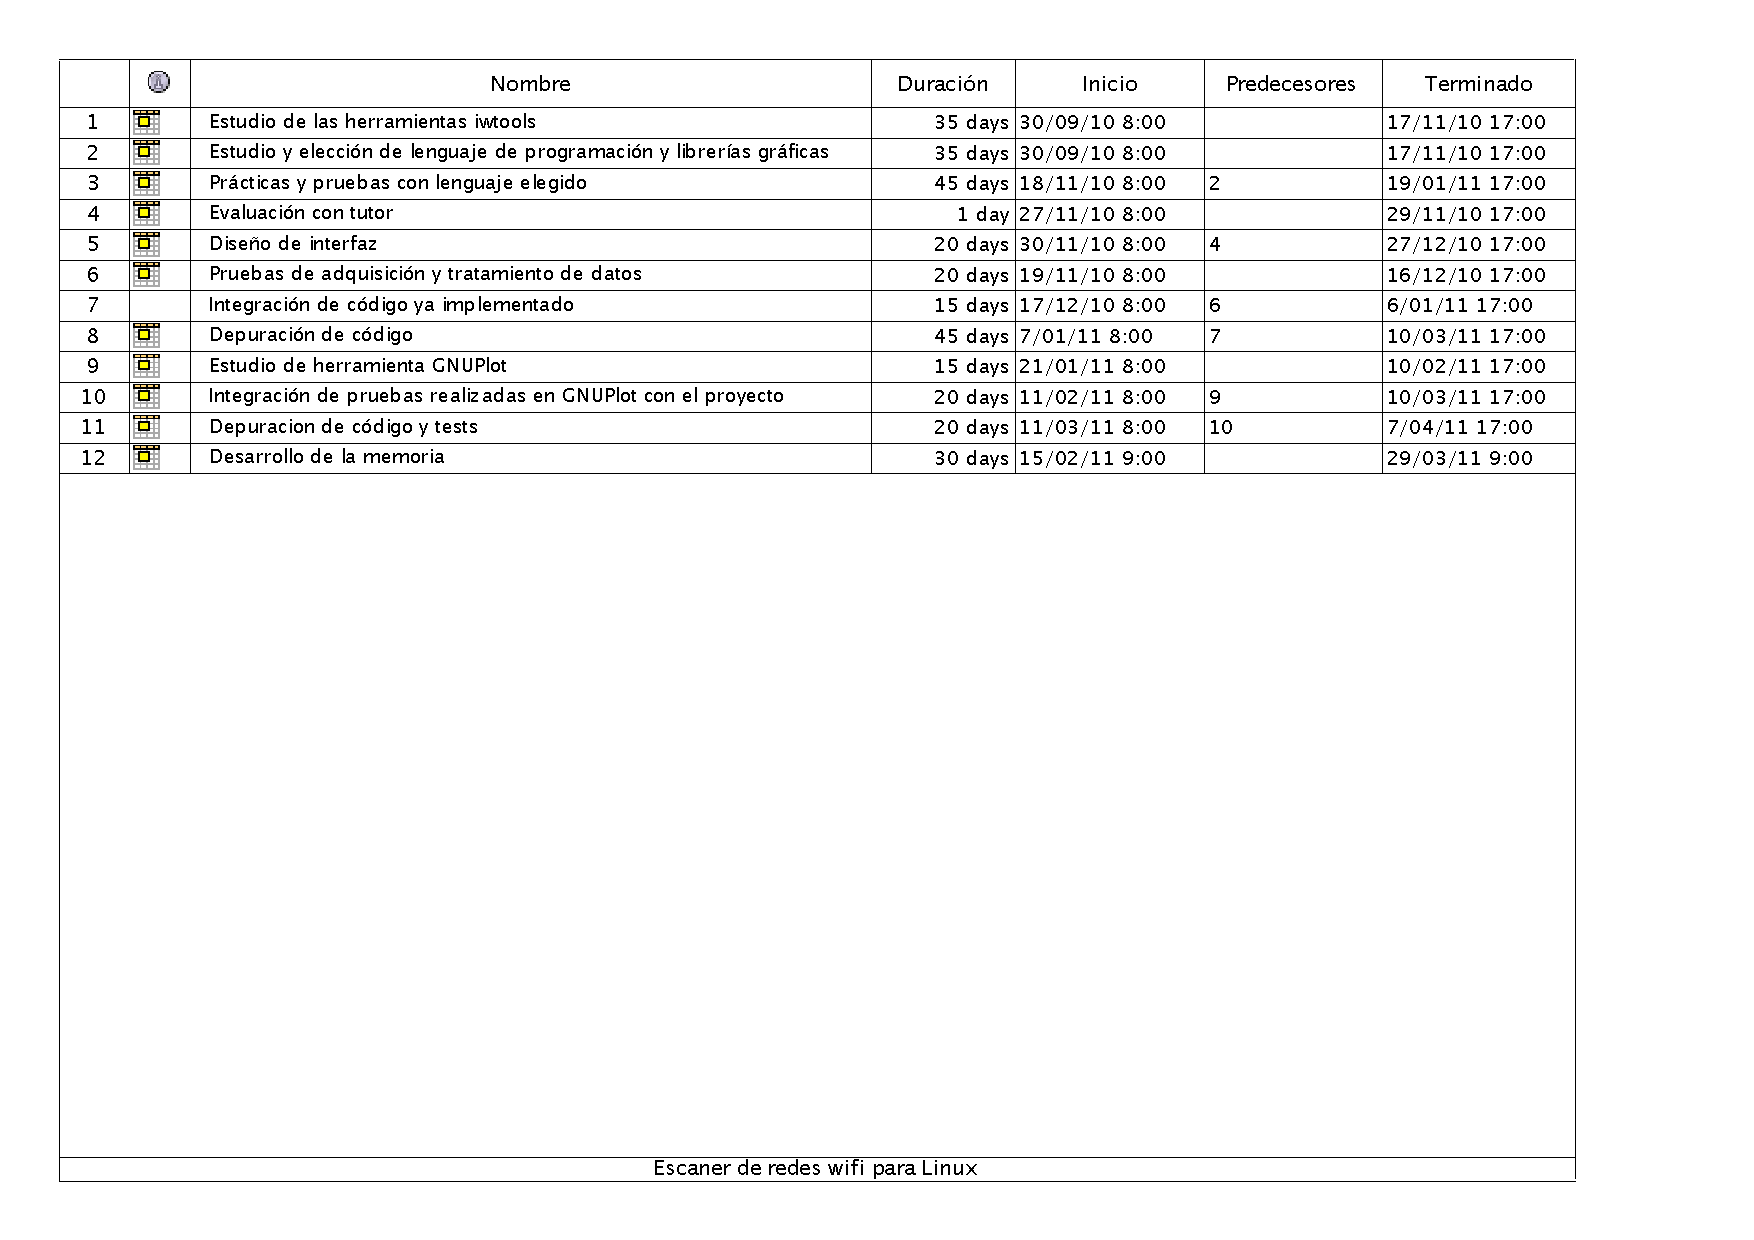
\includepdf[]{src/planificacion_por_hitos.pdf}
 \newpage{\pagestyle{empty}\cleardoublepage} 
    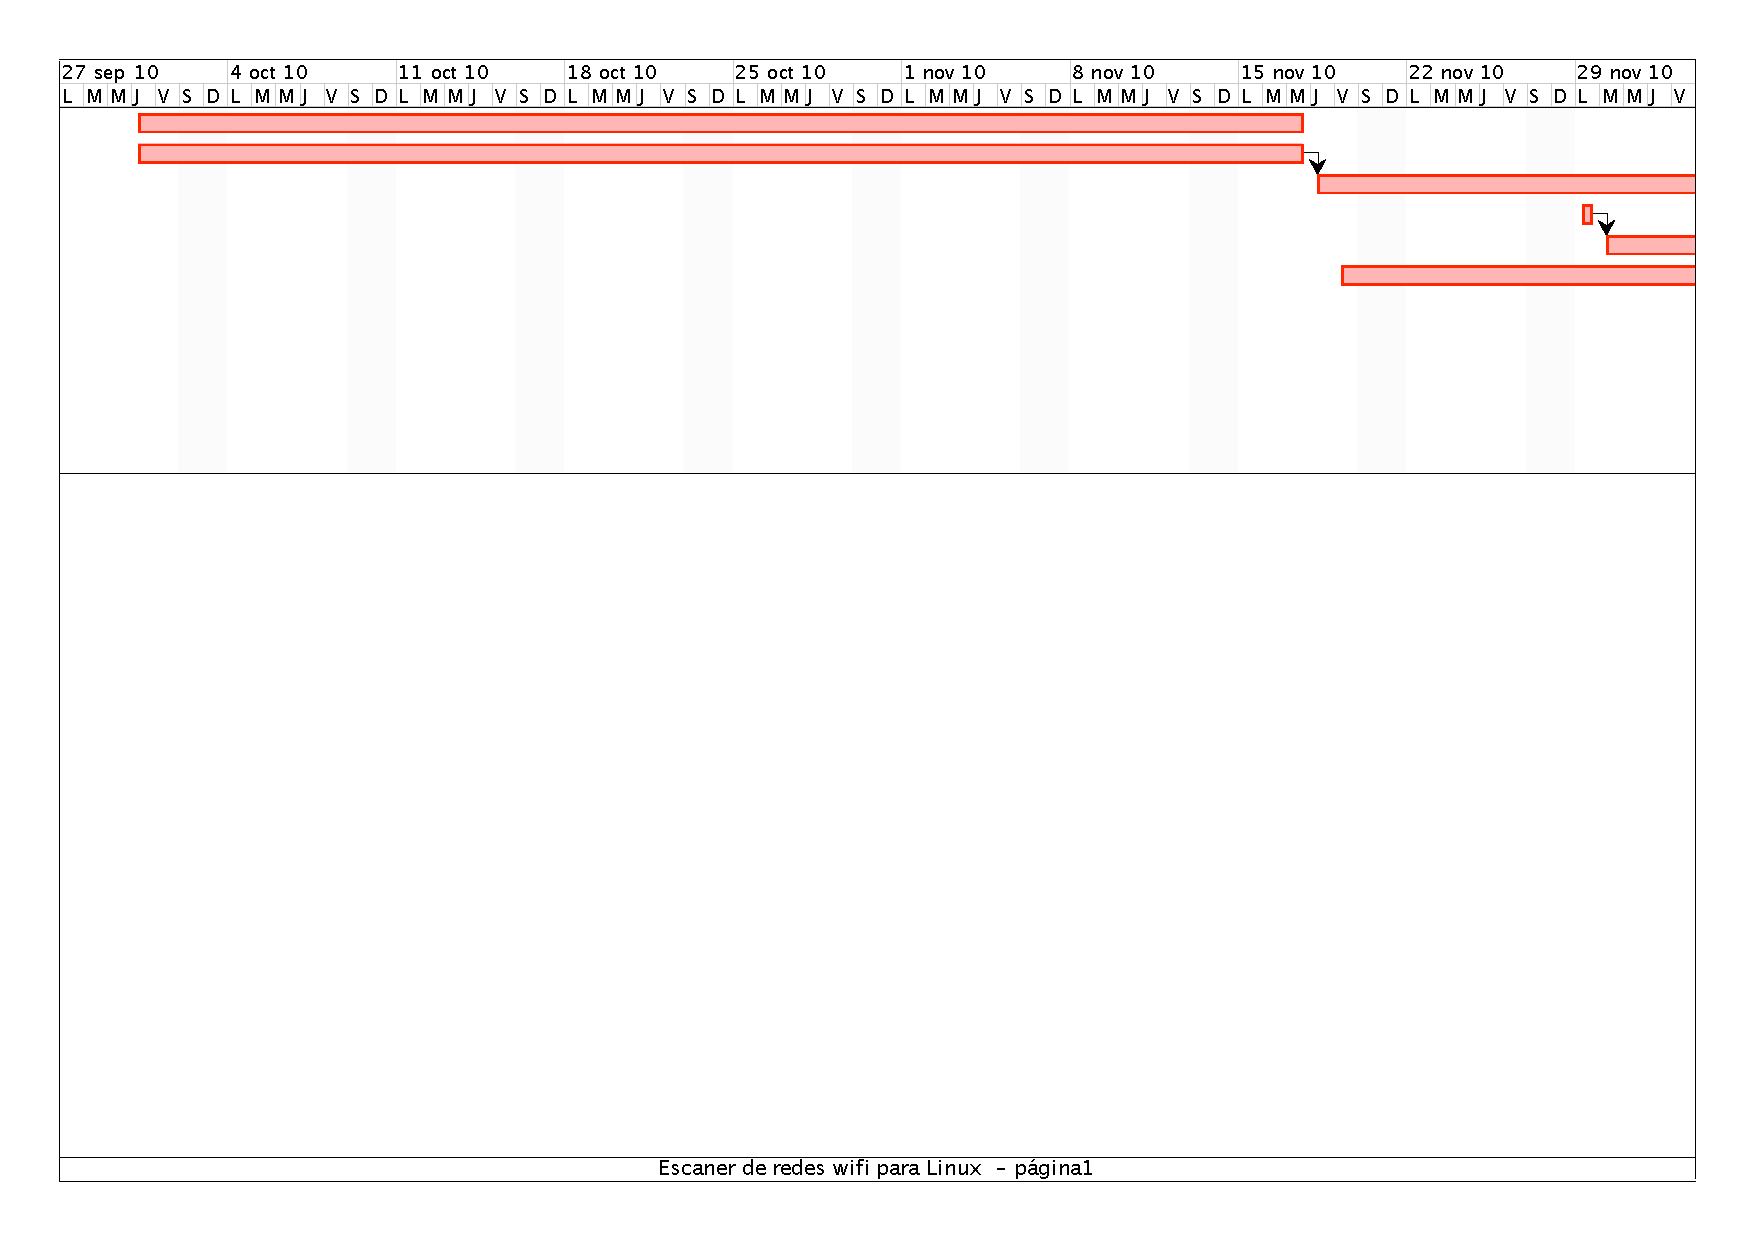
\includepdf[pages={1-3}, landscape]{src/planificacion_gantt.pdf}
 \newpage{\pagestyle{empty}\cleardoublepage} 

\section*{Presupuesto}

A partir de la duraci�n prevista de las tareas a realizar y el coste de los materiales utilizados, se puede obtener el coste de desarrollo del proyecto. Este coste ser� aproximado ya que es previo a la realizaci�n del mismo.\\

Un coste importante es el que deriva del sueldo de los trabajadores implicados en �l. En este caso, se trata de un �nico trabajador (el alumno). Para determinar el sueldo de este trabajador, se supone que se trata de un ingeniero t�cnico ya que es la titulaci�n en la cual se est� desarrollando el proyecto. Esto explica por qu� se ha planificado en 180 d�as (6 meses) y no en 90.\\

El sueldo mensual de un ingeniero t�cnico se supondr� de 1200 euros a jornada completa de 8 horas. Por lo tanto el trabajador ganar�a en torno a los 7.5 euros/hora. Este proyecto se ha realizado a media jornada,debido a la compaginaci�n con otros trabajos.\\

Con este c�lculo, se puede obtener el sueldo total del trabajador teniendo sabiendo que el proyecto tendr� una duraci�n de 720 horas. \\
720 x 7.5 = 5400\euro . Este ser� el sueldo del trabajador.

Tomando �ste proyecto desde cero, la inversi�n f�sica a realizar no es muy elevada. Se comenz� el desarrollo en un pc obsoleto, sin conexi�n v�a wi-fi, por lo que hubo que adquirir una tarjeta USB. A continuaci�n se detallan los costes del desarrollo:\\

\begin{center}
\begin{table}[h]
\begin{tabular}{|c||c|}
\hline \rule[-2ex]{0pt}{5.5ex} \textbf{Elemento} & Precio \\ 
\hline 
\hline \rule[-2ex]{0pt}{5.5ex} Libro C++ GUI Programming with Qt 4 &  40 \euro \\ 
\hline \rule[-2ex]{0pt}{5.5ex} Libro Foundations of Qt Development  & 33\euro \\ 
\hline \rule[-2ex]{0pt}{5.5ex} Herramientas Qt & 0\euro \\ 
\hline \rule[-2ex]{0pt}{5.5ex} Herramientas IwTools & 0\euro \\ 
\hline \rule[-2ex]{0pt}{5.5ex} Gnuplot & 0\euro \\ 
\hline \rule[-2ex]{0pt}{5.5ex} \LaTeX & 0\euro \\ 
\hline \rule[-2ex]{0pt}{5.5ex} Licencia ArchLinux & 0\euro \\ 
\hline \rule[-2ex]{0pt}{5.5ex} Horas de desarrollo & 180 d�as*7,5\euro /hora* 4 horas/d�a = 5400\euro \\ 
\hline \rule[-2ex]{0pt}{5.5ex} USB D--Link DWT  & 19,95\euro \\ 
\hline 
\hline \rule[-2ex]{0pt}{5.5ex} \textbf{total} & \textbf{5492,95\euro} \\ 
\hline 
\end{tabular} 
\caption{Tabla de presupuesto}
\label{Tabla de presupuesto}
\end{table}
\end{center}




\chapter{Especificaci�n de requisitos}
%DESARROLLO Y UML

\section{Desarrollo del proyecto}

Para la realizaci�n de este proyecto se han seguido una serie de pasos de forma cronol�gica:
\begin{enumerate}
\item \underline{Aprendizaje de interfaces gr�ficas}\\
En primer lugar, se estudio el c�digo de iwconfig, para tratar de integrar el comando dentro del proyecto, se pretend�a hacer que el programa pudiera conectar a una red seleccionada, pero para ello se necesitan privilegios de administrador, por tanto, se descart� esta posibilidad. Tambi�n se consider� integrar el c�digo de iwlist junto al c�digo del proyecto, pero se descarto esta opci�n para simplificar el c�digo.\\

Al mismo tiempo, se lleva a cabo un aprendizaje de funcionamiento de varias librer�as gr�ficas para, junto con el lenguaje a utilizar, llevar a cabo el desarrollo del proyecto. Se descart� Java como lenguaje en detrimento de C/C++ o Python y se empez� a realizar pruebas en C con GTK+, pero fue descartado al pasar a utilizar C++ por dificultades en su integraci�n. Finalmente, se eligi� C++ y las librer�as Qt\footnote{http://qt.nokia.com/}.Se realizan varias pruebas para practicar con la interactuaci�n de widgets --una de las principales caractr�sticas de Qt-- con ejemplos sencillos, como unir el valor de un spinbox con una barra deslizante \ver{prueba1}.\\ 

\figura{0.5}{imgs/capturas/ejemplopruebas.png}{Prueba con widgets de Qt}{prueba1}{h}


\item \underline{Pruebas con las herramientas elegidas}\\

Tras comunicar al tutor la elecci�n del lenguaje y las librer�as gr�ficas, se procedi� a realizar un primer dise�o de la interfaz gr�fica. Esta se pretend�a hacerla lo m�s similar posible a la interfaz del programa original (NetSurveyor), pero la interactividad en la selecci�n de las redes y los gr�ficos mostrados se dejaron para futuras ampliaciones del proyecto.\\	

\figura{0.7}{imgs/capturas/netsurveyor.png}{Vista del programa NetSurveyor}{netsurveyor}{h}


Durante el an�lisis y desarrollo del proyecto, se estudi� el lenguaje Java, pero al no contar el alumno con experiencia en este lenguaje ni haber realizado ninguna interfaz gr�fica, se decidi� descartar el lenguaje para acortar la fase de desarrollo. Sin embargo, se pretend�a que el proyecto fuese ampliable a otras plataformas (Windows, Mac Os X\ldots), as� que se decidi� utilizar C++ que, junto a las librer�as Qt, satisfac�an esta premisa.\\

Se realizaron pruebas sencillas con la librer�a Qt, interacci�n entre widgets \ver{prueba1} , mostrar elementos en tablas, lectura/escritura en ficheros. Con estas pruebas se fue directo al grano en el desarrollo del proyecto.
 Esto supuso un c�mulo de problemas que se tuvo que estudiar la soluci�n, el principal problema fue que el escaneo lo tenia que hacer de forma continua, bloqueando el resto del programa y haciendo que el sistema se volviera muy lento. Para solucionar �ste problema, se estudi� el cap�tulo 14 del libro \cite{Blanchette}, multithreading, y comunicando el thread creado con la interfaz principal.\\

\item \underline{Dise�o de la interfaz}\\

La interfaz fue dise�ada siguiendo el dise�o del programa NetSurveyor, por lo que en este punto, no hubo dificultad al realizar el dise�o. El IDE QtCreator incorpora en su interfaz un apartado para esta tarea. Tambi�n existe el IDE QtDesigner, que combinado con QDevelop, realiza la misma tarea que QtCreator, as� pues, podr�amos considerar QtCreator como una suite de programacion Qt.\\

\item \underline{Adquisici�n de datos}\\
Para la adquisici�n de datos desde el comando \textit{iwlist wlan0 scan} se prefiri� utilizar un comando de ejecuci�n de procesos, volcando los resultados en un fichero. Esto facilitar� posteriormente la elecci�n de la tarjeta wi-fi y la posibilidad de actualizaci�n de las herramientas iwtools.\\
El principal problema al tomar los datos fue que se us� el descriptor stdin ($>>$), el cual da la facilidad de poder tomar los datos por separado, ya que considera los espacios como separadores. Esto supone un problema cuando el ESSID (el nombre de la red) contiene varias palabras, ya que s�lo toma la primera de ellas. Se descubri� que hay un flag que evita que corte el flujo de datos por lectura de espacios, noskipws (no skip white spaces), se realizaron pruebas con �ste flag pero no resultaron satisfactorias, el c�digo no le�a correctamente la ESSID. Finalmente, se decidi� optar por utilizar la funci�n getline\footnote{istream\& getline (char* s, streamsize n, char delim );}.
Tambi�n se definieron dos funciones, una para cortar una cadena `split'\footnote{void splitstring(string str, string separator, string \&first, string \&second);} y otra para desechar la primera parte de la cadena `limpiar'\footnote{void limpiar(string str, string separator, string \&resultado);}. \\

\item \underline{Integraci�n del c�digo en el proyecto}\\

La integraci�n del la adquisici�n de datos con el del dise�o de la interfaz descubri� un problema que no se hab�a tenido en cuenta, el escaneo continuo de la tarjeta wi-fi bloqueaba el flujo normal del programa. Esto hizo necesario incorporar un thread al programa, el cual ser� el encargado de realizar esta tarea.\\
Esto produjo una parada en el desarrollo del proyecto, no se hab�a tenido en cuenta esta estrategia y tuvo que estudiarse c�mo programar threads. Para ello, se estudi� el cap�tulo 14 del libro C++ GUI Programming with Qt4\cite{Blanchette}.\\

\figura{0.9}{imgs/capturas/threads.png}{Ejemplo de uso de threads del libro usado}{threads}{h}

Una vez solucionado �ste problema, se procedi� a mostrar los datos en una lista tipo TreeView, generar los gr�ficos, los informes (pdf y html)\ldots Para mostrar los datos en el TreeView, se encontraron dificultades debido a que se necesitaba crear un model est�ndar de item, pero no se consegu�a que mostrara los datos, as� pues, se estudio el cap�tulo de tablas y listas del libro \cite{Thelin}. Finalmente, se descubri� que se necesitaba crear un QItemDelegate.La clase QItemDelegate proporciona una visualizaci�n y funciones de edici�n de elementos de datos de un modelo.
QItemDeleate se puede utilizar para proporcionar caracter�sticas personalizadas y mostrar widgets de editor de visas de elementos basados en subclases QAbstractItemView. El uso de un delegado para este prop�sito permite que los mecanismos de visualizaci�n y edici�n para personalizar sean desarrollados de forma independiente del modelo y la vista.\\

Cuando se muestran los elementos de un modelo personalizado en una vista est�ndar, se garantiza que el modelo devuelve los datos adecuados para cada uno de los roles que determinan la aparici�n de los elementos en las vistas. El delegado por defecto utilizado por las vistas est�ndar de Qt utiliza esta informaci�n de las funciones para mostrar los elementos en la mayor�a de las formas m�s comunes que exigen los usuarios. \\


\lstinputlisting[language=c++,caption={ItemDelegate implementado en el c�digo}]{src/itemDelegate.h}


\item \underline{Estudio de Gnuplot}\\
Para estudio de GnuPlot se decidi� hacer pruebas de gr�ficos con una bater�a de datos ya preparados, se limit� el uso de �ste a generar dos scripts que prepara el programa para realizar los gr�ficos resultantes y dos ficheros con los datos a mostrar.\\

\lstinputlisting[language=java,caption={Ejemplo de script para Gnuplot}]{src/gnuplot1.plt}


El resultado de estos scripts son los gr�ficos de la potencia de las se�ales y el uso de los canales.\\

\item \underline{Tests}\\
Se procedi� a las pruebas de la aplicaci�n en diversos lugares, tanto en la Universidad, como en la biblioteca municipal de Onda, en casa del alumno con las redes de los vecinos y a�adiendo routers wi-fi desechados, en cafeter�as con servicio wi-fi \ldots Se procedi� al an�lisis de los datos y se encontr� un problema extra�o, la lectura de la se�al a veces lee valores incorrectos. La primera hip�tesis fue un error de programaci�n en la lectura de ese dato, y se procedi� a analizar (se especulaba que tomaba el valor negativo de forma incorrecta), pero no se encontr� el error. Se procedi� entonces a realizar pruebas sin la llamada al procesi \textit{iwlist wlan0 scan}, utilizando una captura de datos previa. Esto deber�a permitir contrastar la hip�tesis y, por tanto, solucionar este problema. No se encontr� el error, pero la aplicaci�n segu�a leyendo de vez en cuando valores extra�os.\\


\figura{0.9}{imgs/capturas/capturaerronea2.png}{Vista de una lectura err�nea}{erronea}{}
\figura{0.9}{imgs/capturas/capturaerronea.png}{Vista de una lectura err�nea}{erronea2}{}

Tras varias pruebas de depuraci�n, se advirti� que las redes que en alg�n momento hab�an sido registradas y que en posteriores lecturas no aparec�an, su vector de se�ales no siempre actualizaba su elemento a�adiendo un 0 al instante de la lectura, siendo de distinto tama�o al resto de vectores, con lo que, en ocasiones, provocaba una lectura de valores err�neos debido a que el vector apuntaba a una direcci�n de memoria incorrecta.\\
\end{enumerate} 


\chapter{Caso de uso}

\section{Diagrama de casos de uso}

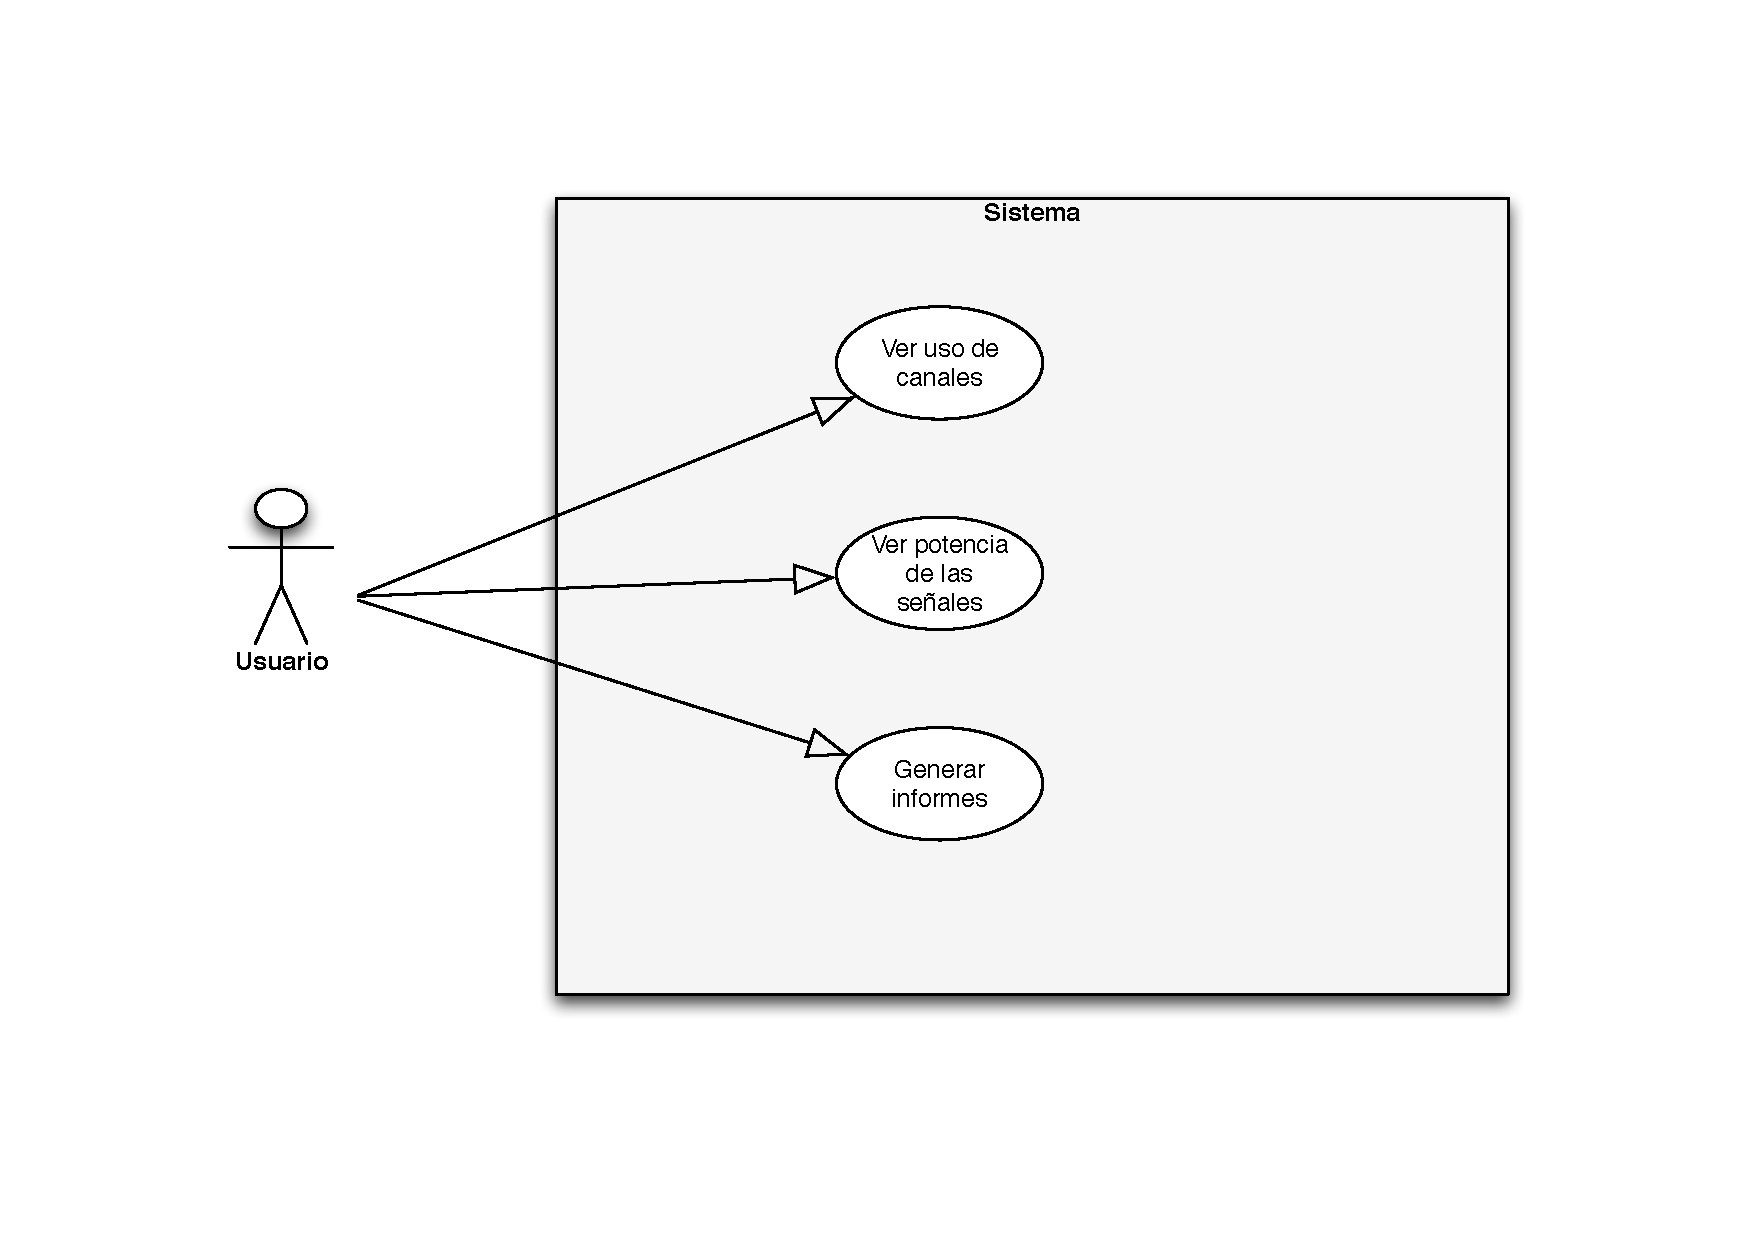
\includegraphics[scale=0.7, angle=90]{src/proyectoCDU.pdf}


%
%\subsection*{Descripci�n de caso de uso}
%
%\begin{center}
%\footnotesize
%\centering\makebox[0cm][c]{
%\begin{tabular}{p{4.1cm}|p{12cm}}
%\hline
%\multicolumn{2}{c}{\textbf{Descripci�n de caso de uso}} \\
%\hline \hline
%\textbf{Identificador} & CU$<$identificador num�rico del caso de uso$>$ \\
%\textbf{Nombre} & $<$nom curt del requisit funcional que descriu el cas d'�s, frase curta amb el verb en actiu$>$ \\
%\hline
%\textbf{Versi�} & $<$versi�	 del requisit$>$ \\
%\textbf{Autors} & $<$nom de l'enginyer de l'empresa que ha realitzat la descripci� del cas d'�s$>$ \\
%\textbf{Fonts} & $<$quina persona o departament de l'empresa, PSI, o quines normes o lleis han originat aquest cas d'�s$>$ \\
%\hline
%\textbf{Descripci�} & El sistema ha de ... $<$descripci� detallada de la funcionalitat que descriu el cas d'�s, objectiu del cas d'�s dins del context$>$ \\
%\textbf{Abast} & $<$determinar el l�mit del requisit$>$ \\
%\textbf{Nivell} & (resum, tasca principal, subtasca) \\
%\textbf{Actor principal} & $<$nom de l'actor que desencadena l'acci� i per al qual el cas d'�s t� major valor afegit, obligatori$>$ \\
%\textbf{Actors secundaris} & $<$altres actors que interactuen amb el cas d'�s, opcional$>$ \\
%\textbf{Relacions} & $<$casos d'�s relacionats$>$ \\
%\hline
%\textbf{Precondici�} & $<$condicions que s'han de donar al sistema abans de l'execuci� del cas d'�s$>$ \\
%\textbf{Condici� fi amb �xit} & $<$condicions que complir� el sistema si el cas d'�s finalitza de forma satisfact�ria$>$ \\
%\textbf{Condici� fi amb frac�s} & $<$condicions que complir� el sistema si el cas d'�s finalitza de forma an�mala$>$ \\
%\textbf{Trigger} & $<$esdeveniment que desencadena l'execuci� del cas d'�s$>$ \\
%\hline
%\textbf{Seq��ncia normal} &	\textbf{Acci�} \\
%\hline
%\hfill \textbf{1} & $<$detall d'acci� 1$>$ \\
%\hfill \textbf{2} & $<$detall d'acci� 2$>$ \\
%\hfill \textbf{2.1} & $<$detall d'acci� 2.1$>$ \\
%\hfill \textbf{2.2} & $<$detall d'acci� 2.2$>$ \\
%\hfill ... &	... \\
%\hline
%\textbf{Excepcions $<$acci� 1$>$} & \textbf{Excepci�} \\
%\hline
%\hfill \textbf{1} & $<$detall d'excepci� 1$>$ \\
%\hfill \textbf{1.1} & $<$detall d'excepci� 1.1$>$ \\
%\hfill \textbf{1.2} & $<$detall d'excepci� 1.2$>$ \\
%\hfill ... &	... \\
%\hline
%\textbf{Excepcions $<$acci� 2.2$>$} & \textbf{Excepci�} \\
%\hline
%\hfill \textbf{1} & $<$detall d'excepci� 1$>$ \\
%\hfill \textbf{2} & $<$detall d'excepci� 2$>$ \\
%\hfill \textbf{3} & $<$detall d'excepci� 3$>$ \\
%\hfill ... &	... \\
%\hline
%\textbf{Freq��ncia esperada} &	$<$n�mero de vegades per unitat de temps (dies, setmanes, mesos, etc.) que s'utilitza aquesta funcionalitat$>$ \\
%\textbf{Import�ncia} & (necessari, desitjable, no vital) \\
%\textbf{Prioritat} & (curt termini, mig termini, llarg termini) \\
%\textbf{Comentaris} & $<$comentaris o observacions addicionals$>$ \\
%\hline
%\end{tabular}}
%\end{center}


\chapter{Conclusiones}
\section{Conclusiones}

El resultado de este proyecto ha resultado muy interesante. Al crearlo desde el principio se ha tenido que realizar una planificaci�n sobre los pasos a seguir y se han tenido que tomar decisiones que afectaban a la realizaci�n del mismo, como la elecci�n del lenguaje de programaci�n o las librer�as gr�ficas a utilizar, pero todo ello sin perder de vista la premisa principal, debe ser extendible a otras plataformas.\\

A pesar de los problemas que han aparecido durante el desarrollo del proyecto, problemas con las librer�as, con la adquisici�n de datos, etc\ldots resulta gratificante ver que el proyecto es funcional y que se han logrado los objetivos establecidos.\\


A nivel personal, decir que he disfrutado en la realizaci�n del proyecto y que los conocimientos adquiridos en programaci�n de \guis abren un abanico de posibilidades para el desarrollo de aplicaciones, un campo que no ha sido estudiado en la carrera y que es casi obligatorio en el �mbito empresarial.\\

%COMENTAR EXPERIENCIAS SOBRE EL PROYECTO Y SU ADECUACION AL MISMO EN LA CARRERA \\
%
%\begin{LARGE}
%FALTA DESARROLLAR\\
%\end{LARGE}


\bibliografia{referencias}
%\bibliografiaOtras{otrasreferencias} %Opcional

% Ap�ndices
\backmatter
\appendix
%\chapter{Acr�nimos}
%
\section{Secci�n} 

El veloz murci�lago hind� com�a feliz cardillo y kiwi.  La cig�e�a tocaba el saxof�n detr�s del palenque de paja.  El veloz murci�lago hind� com�a feliz cardillo y kiwi.  La cig�e�a tocaba el saxof�n detr�s del palenque de paja.  El veloz murci�lago hind� com�a feliz cardillo y kiwi.


\begin{table}
\begin{center}
\begin{tabular}{|c|c|c|}
\hline Codigo & Nombre & Apellidos \\ 
\hline\hline 1 & Fulanito & P� \\ 
\hline 2 & Menganita & P� \\ 
\hline 3 & Miguel & Campoviejo \\ 
\hline 4 & Kepa & Sakolegi \\ 
\hline 
\end{tabular} 
\caption{Esto es una tabla}
\label{tbTabla1}
\end{center}
\end{table}

El veloz murci�lago hind� com�a feliz cardillo y kiwi.  La cig�e�a tocaba el saxof�n detr�s del palenque de paja.  El veloz murci�lago hind� com�a feliz cardillo y kiwi.  La cig�e�a tocaba el saxof�n detr�s del palenque de paja.  El veloz murci�lago hind� com�a feliz cardillo y kiwi. El veloz murci�lago hind� com�a feliz cardillo y kiwi.  La cig�e�a tocaba el saxof�n detr�s del palenque de paja.  El veloz murci�lago hind� com�a feliz cardillo y kiwi.  La cig�e�a tocaba el saxof�n detr�s del palenque de paja.  El veloz murci�lago hind� com�a feliz cardillo y kiwi.

El veloz murci�lago hind� com�a feliz cardillo y kiwi.  La cig�e�a tocaba el saxof�n detr�s del palenque de paja.  El veloz murci�lago hind� com�a feliz cardillo y kiwi.  La cig�e�a tocaba el saxof�n detr�s del palenque de paja.  El veloz murci�lago hind� com�a feliz cardillo y kiwi.

\figura{0.4}{imgs/logo.png}{Esto es una imagen}{figImagen1}{}

\section{Secci�n} 

El veloz murci�lago hind� com�a feliz cardillo y kiwi.  La cig�e�a tocaba el saxof�n detr�s del palenque de paja.  El veloz murci�lago hind� com�a feliz cardillo y kiwi.  La cig�e�a tocaba el saxof�n detr�s del palenque de paja.  El veloz murci�lago hind� com�a feliz cardillo y kiwi. El veloz murci�lago hind� com�a feliz cardillo y kiwi.  La cig�e�a tocaba el saxof�n detr�s del palenque de paja.  El veloz murci�lago hind� com�a feliz cardillo y kiwi.  La cig�e�a tocaba el saxof�n detr�s del palenque de paja.  El veloz murci�lago hind� com�a feliz cardillo y kiwi.

\figura{0.4}{imgs/logo.png}{Esto es una imagen}{figImagen2}{}

\begin{table}
\begin{center}
\begin{tabular}{|c|c|c|}
\hline Codigo & Nombre & Apellidos \\ 
\hline\hline 1 & Fulanito & P� \\ 
\hline 2 & Menganita & P� \\ 
\hline 3 & Miguel & Campoviejo \\ 
\hline 4 & Kepa & Sakolegi \\ 
\hline 
\end{tabular} 
\caption{Esto es una tabla}
\label{tbTabla2}
\end{center}
\end{table}

El veloz murci�lago hind� com�a feliz cardillo y kiwi.  La cig�e�a tocaba el saxof�n detr�s del palenque de paja.  El veloz murci�lago hind� com�a feliz cardillo y kiwi.  La cig�e�a tocaba el saxof�n detr�s del palenque de paja.  El veloz murci�lago hind� com�a feliz cardillo y kiwi.

El veloz murci�lago hind� com�a feliz cardillo y kiwi.  La cig�e�a tocaba el saxof�n detr�s del palenque de paja.  El veloz murci�lago hind� com�a feliz cardillo y kiwi.  La cig�e�a tocaba el saxof�n detr�s del palenque de paja.  El veloz murci�lago hind� com�a feliz cardillo y kiwi.

\figura{0.5}{imgs/logo.png}{Esto es una imagen}{figImagen3}{}

El veloz murci�lago hind� com�a feliz cardillo y kiwi.  La cig�e�a tocaba el saxof�n detr�s del palenque de paja.  El veloz murci�lago hind� com�a feliz cardillo y kiwi.  La cig�e�a tocaba el saxof�n detr�s del palenque de paja.  El veloz murci�lago hind� com�a feliz cardillo y kiwi.

\section{Secci�n} 

El veloz murci�lago hind� com�a feliz cardillo y kiwi.  La cig�e�a tocaba el saxof�n detr�s del palenque de paja.  El veloz murci�lago hind� com�a feliz cardillo y kiwi.  La cig�e�a tocaba el saxof�n detr�s del palenque de paja.  El veloz murci�lago hind� com�a feliz cardillo y kiwi. El veloz murci�lago hind� com�a feliz cardillo y kiwi.  La cig�e�a tocaba el saxof�n detr�s del palenque de paja.  El veloz murci�lago hind� com�a feliz cardillo y kiwi.  La cig�e�a tocaba el saxof�n detr�s del palenque de paja.  El veloz murci�lago hind� com�a feliz cardillo y kiwi.

\begin{table}
\begin{center}
\begin{tabular}{|c|c|c|}
\hline Codigo & Nombre & Apellidos \\ 
\hline\hline 1 & Fulanito & P� \\ 
\hline 2 & Menganita & P� \\ 
\hline 3 & Miguel & Campoviejo \\ 
\hline 4 & Kepa & Sakolegi \\ 
\hline 
\end{tabular} 
\caption{Esto es una tabla}
\label{tbTabla3}
\end{center}
\end{table}

El veloz murci�lago hind� com�a feliz cardillo y kiwi.  La cig�e�a tocaba el saxof�n detr�s del palenque de paja.  El veloz murci�lago hind� com�a feliz cardillo y kiwi.  La cig�e�a tocaba el saxof�n detr�s del palenque de paja.  El veloz murci�lago hind� com�a feliz cardillo y kiwi.

\figura{0.5}{imgs/logo.png}{Esto es una imagen}{figImagen4}{}

El veloz murci�lago hind� com�a feliz cardillo y kiwi.  La cig�e�a tocaba el saxof�n detr�s del palenque de paja.  El veloz murci�lago hind� com�a feliz cardillo y kiwi.  La cig�e�a tocaba el saxof�n detr�s del palenque de paja.  El veloz murci�lago hind� com�a feliz cardillo y kiwi.

\begin{codigo}
public void postCreate(GridContext context) throws GridServiceException
\{
    // Create Service Data Element
    serviceData = this.getServiceDataSet().create("MathData");

    // Set the value of the SDE to a MathDataType instance
    mathData = new MathDataType();
    serviceData.setValue(mathData);

    // Set intial values of MathServiceData
    mathData.setLastOp("NONE");
    mathData.setNumOps(0);

    // Add SDE to Service Data Set
    this.getServiceDataSet().add(serviceData);
\}
\end{codigo}

El veloz murci�lago hind� com�a feliz cardillo y kiwi.  La cig�e�a tocaba el saxof�n detr�s del palenque de paja.  El veloz murci�lago hind� com�a feliz cardillo y kiwi.  La cig�e�a tocaba el saxof�n detr�s del palenque de paja.  El veloz murci�lago hind� com�a feliz cardillo y kiwi. El veloz murci�lago hind� com�a feliz cardillo y kiwi.  La cig�e�a tocaba el saxof�n detr�s del palenque de paja.  El veloz murci�lago hind� com�a feliz cardillo y kiwi.  La cig�e�a tocaba el saxof�n detr�s del palenque de paja.  El veloz murci�lago hind� com�a feliz cardillo y kiwi.

\figura{0.5}{imgs/logo.png}{Esto es una imagen}{figImagen5}{}
\figura{0.4}{imgs/logo.png}{Esto es una imagen}{figImagen6}{}

El veloz murci�lago hind� com�a feliz cardillo y kiwi.  La cig�e�a tocaba el saxof�n detr�s del palenque de paja.  El veloz murci�lago hind� com�a feliz cardillo y kiwi.  La cig�e�a tocaba el saxof�n detr�s del palenque de paja.  El veloz murci�lago hind� com�a feliz cardillo y kiwi.

El veloz murci�lago hind� com�a feliz cardillo y kiwi.  La cig�e�a tocaba el saxof�n detr�s del palenque de paja.  El veloz murci�lago hind� com�a feliz cardillo y kiwi.  La cig�e�a tocaba el saxof�n detr�s del palenque de paja.  El veloz murci�lago hind� com�a feliz cardillo y kiwi.

\section{Secci�n} 


El veloz murci�lago hind� com�a feliz cardillo y kiwi.  La cig�e�a tocaba el saxof�n detr�s del palenque de paja.  El veloz murci�lago hind� com�a feliz cardillo y kiwi.  La cig�e�a tocaba el saxof�n detr�s del palenque de paja.  El veloz murci�lago hind� com�a feliz cardillo y kiwi. El veloz murci�lago hind� com�a feliz cardillo y kiwi.  La cig�e�a tocaba el saxof�n detr�s del palenque de paja.  El veloz murci�lago hind� com�a feliz cardillo y kiwi.  La cig�e�a tocaba el saxof�n detr�s del palenque de paja.  El veloz murci�lago hind� com�a feliz cardillo y kiwi.

\begin{table}
\begin{center}
\begin{tabular}{|c|c|c|}
\hline Codigo & Nombre & Apellidos \\ 
\hline\hline 1 & Fulanito & P� \\ 
\hline 2 & Menganita & P� \\ 
\hline 3 & Miguel & Campoviejo \\ 
\hline 4 & Kepa & Sakolegi \\ 
\hline 
\end{tabular} 
\caption{Esto es una tabla}
\label{tbTabla4}
\end{center}
\end{table}

El veloz murci�lago hind� com�a feliz cardillo y kiwi.  La cig�e�a tocaba el saxof�n detr�s del palenque de paja.  El veloz murci�lago hind� com�a feliz cardillo y kiwi.  La cig�e�a tocaba el saxof�n detr�s del palenque de paja.  El veloz murci�lago hind� com�a feliz cardillo y kiwi.

El veloz murci�lago hind� com�a feliz cardillo y kiwi.  La cig�e�a tocaba el saxof�n detr�s del palenque de paja.  El veloz murci�lago hind� com�a feliz cardillo y kiwi.  La cig�e�a tocaba el saxof�n detr�s del palenque de paja.  El veloz murci�lago hind� com�a feliz cardillo y kiwi.

\figura{0.5}{imgs/logo.png}{Esto es una imagen}{figImagen7}{}

\newpage
%\lstinputlisting[language=Java,caption={Otro formato de c�digo fuente}]{src/Prueba.java}
\codigofuente{Java}{Otro formato de c�digo fuente}{src/Prueba.java}

%\chapter{Instalaci�n}
%Para compilar �ste proyecto se necesita satisfacer una serie de dependencias del c�digo. �stas se obtienen mediante el comando LDD, as� pues, obtenemos esta lista de dependencias del proyecto;
\begin{enumerate}
\item 	linux-vdso.so.1 =>  (0x00007fff3f7d8000)
\item 	libQtGui.so.4 => /usr/lib/libQtGui.so.4 (0x00007f03613ac000)
\item 	libQtCore.so.4 => /usr/lib/libQtCore.so.4 (0x00007f0360f1e000)
\item 	libpthread.so.0 => /lib/libpthread.so.0 (0x00007f0360d01000)
\item 	libstdc++.so.6 => /usr/lib/libstdc++.so.6 (0x00007f03609f7000)
\item 	libgcc_s.so.1 => /usr/lib/libgcc_s.so.1 (0x00007f03607e1000)
\item 	libc.so.6 => /lib/libc.so.6 (0x00007f0360480000)
\item 	libglib-2.0.so.0 => /usr/lib/libglib-2.0.so.0 (0x00007f0360199000)
\item 	libpng14.so.14 => /usr/lib/libpng14.so.14 (0x00007f035ff70000)
\item 	libz.so.1 => /usr/lib/libz.so.1 (0x00007f035fd58000)
\item 	libfreetype.so.6 => /usr/lib/libfreetype.so.6 (0x00007f035fabf000)
\item 	libgobject-2.0.so.0 => /usr/lib/libgobject-2.0.so.0 (0x00007f035f870000)
\item 	libSM.so.6 => /usr/lib/libSM.so.6 (0x00007f035f669000)
\item 	libICE.so.6 => /usr/lib/libICE.so.6 (0x00007f035f44e000)
\item 	libXrender.so.1 => /usr/lib/libXrender.so.1 (0x00007f035f244000)
\item 	libfontconfig.so.1 => /usr/lib/libfontconfig.so.1 (0x00007f035f010000)
\item 	libXext.so.6 => /usr/lib/libXext.so.6 (0x00007f035edfe000)
\item 	libX11.so.6 => /usr/lib/libX11.so.6 (0x00007f035eac0000)
\item 	libm.so.6 => /lib/libm.so.6 (0x00007f035e83d000)
\item 	libdl.so.2 => /lib/libdl.so.2 (0x00007f035e639000)
\item 	libgthread-2.0.so.0 => /usr/lib/libgthread-2.0.so.0 (0x00007f035e435000)
\item 	librt.so.1 => /lib/librt.so.1 (0x00007f035e22d000)
\item 	/lib/ld-linux-x86-64.so.2 (0x00007f036203e000)
\item 	libpcre.so.0 => /lib/libpcre.so.0 (0x00007f035dff2000)
\item 	libuuid.so.1 => /lib/libuuid.so.1 (0x00007f035ddee000)
\item 	libexpat.so.1 => /usr/lib/libexpat.so.1 (0x00007f035dbc5000)
\item 	libxcb.so.1 => /usr/lib/libxcb.so.1 (0x00007f035d9aa000)
\item 	libXau.so.6 => /usr/lib/libXau.so.6 (0x00007f035d7a8000)
\item 	libXdmcp.so.6 => /usr/lib/libXdmcp.so.6 (0x00007f035d5a3000)
\end{enumerate}

Una vez resueltas estas dependencias, dentro de la carpeta del proyecto CAPTURA DE PANTALLA existe un script de compilaci�n e instalaci�n en el sistema, simplemente hay que escribir el comando;
El programa se instala en entorno Gnome en Aplicaciones; internet
CAPTURA DE PANTALLA


\chapter{C�digo fuente}
\lstinputlisting[language=C++, caption={archivo funciones.cpp}]{src/src/funciones.cpp}
\newpage
\lstinputlisting[language=C++, caption={archivo funciones.h}]{src/src/funciones.h}
\newpage
\lstinputlisting[language=C++, caption={archivo itemDelegate.h}]{src/src/itemDelegate.h}
\newpage
\lstinputlisting[language=C++, caption={archivo main.cpp}]{src/src/main.cpp}
\newpage
\lstinputlisting[language=C++, caption={archivo mainwindow.h}]{src/src/mainwindow.h}
\newpage
\lstinputlisting[language=C++, caption={archivo mainwindow.cpp}]{src/src/mainwindow.cpp}
\newpage
\lstinputlisting[language=C++, caption={archivo thread.h}]{src/src/thread.h}
\newpage
\lstinputlisting[language=C++, caption={archivo thread.cpp}]{src/src/thread.cpp}
\newpage
\lstinputlisting[language=C++, caption={archivo wifiStruct.h}]{src/src/wifiStruct.h}
\newpage
\lstinputlisting[language=XML, caption={archivo mainwindow.ui}]{src/src/mainwindow.ui}




%\bibliografia{referencias}
%\bibliografiaOtras{otrasreferencias} %Opcional



\end{document}
